\autobookmark
\begin{frame}{Simulation has very good agreement with experimental data}
  \begin{columns}[T]

    \begin{column}{.5\textwidth}
      \myonly{1}{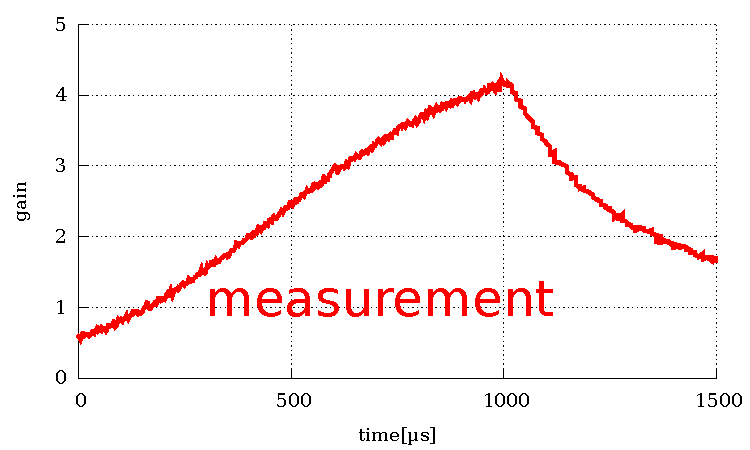
\includegraphics[width=0.5\paperwidth]{graphics/benchmark_results_0.pdf}}
      \myonly{2-}{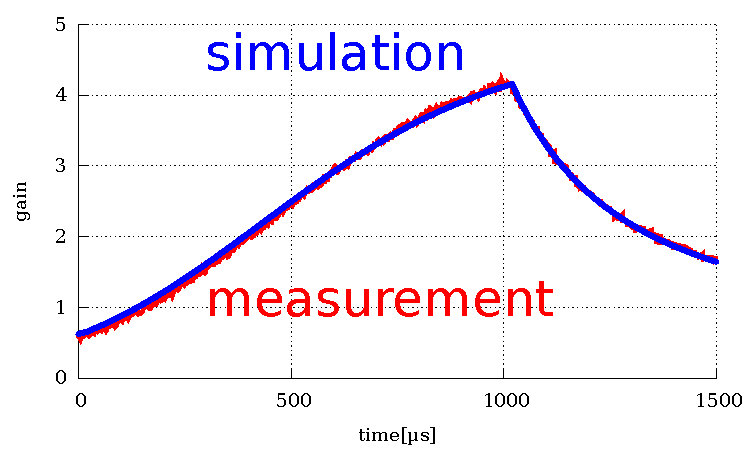
\includegraphics[width=0.5\paperwidth]{graphics/benchmark_results_1.pdf}}
    \end{column}

    \begin{column}{.5\textwidth}
      \begin{itemize}
          \myuncover{1}{3}{
            \item Reminder: plot from experimental data
          }
          \myuncover{2}{3}{
            \item Simulating predicts the experiment very closely
          }
          \myuncover{3}{3}{
            \item Takes about 7h on 1 GPU
          }
      \end{itemize}
    \end{column}

  \end{columns}
\end{frame}

%\begin{frame}{Predefined colours}
%  The template defines a set of colours according to the CD guidelines:\par
%  \begin{itemize}
%      \begin{minipage}[t]{0.5\linewidth}
%      \item \textcolor{hzdr-blue}{Helmholtz Blue}    
%      \item \textcolor{hzdr-orange}{Rossendorf Orange}  
%      \item \textcolor{hzdr-darkblue}{Helmholtz Dark Blue}
%      \item \textcolor{hzdr-gray1}{Gray1}   
%      \item \textcolor{hzdr-gray2}{Gray2}   
%      \item \textcolor{hzdr-gray3}{Gray3}   
%      \item \textcolor{hzdr-struct}{Structure of Matter}  
%      \end{minipage}%
%      \begin{minipage}[t]{0.5\linewidth}
%      \item \textcolor{hzdr-health}{Health}  
%      \item \textcolor{hzdr-energy}{Energy}  
%      \item \textcolor{hzdr-earth}{Earth and Environment}   
%      \item \textcolor{hzdr-keytec}{Key Technologies}  
%      \item \textcolor{hzdr-aero}{Aeronautics, Space and Transport}
%      \end{minipage}
%  \end{itemize}
%\end{frame}

